\documentclass[11pt]{article}

\usepackage[T2A]{fontenc}
\usepackage[utf8]{inputenc}
\usepackage[russian]{babel}

\usepackage{indentfirst}
\usepackage{geometry}

\usepackage{amsmath, amssymb, amsfonts, amsthm, amscd}
\usepackage{mathrsfs}

\usepackage{caption}
\usepackage{graphicx}
\usepackage[all]{xy}

\geometry{a4paper}
\sloppy


\theoremstyle{plain}
\newtheorem*{statement}{Утверждение}
\theoremstyle{definition}
\newtheorem*{definition}{Определение}
\theoremstyle{remark}
\newtheorem*{remark}{Замечание}

\renewcommand{\le}{\leqslant}
\renewcommand{\ge}{\geqslant}
\renewcommand{\phi}{\varphi}
\renewcommand{\epsilon}{\varepsilon}
\renewcommand{\kappa}{\varkappa}

\newcommand{\comdots}{,\!..}
\newcommand{\subdim}[1]{\lfloor \dim #1 \rfloor}

\DeclareMathOperator*{\Hom}{Hom}
\DeclareMathOperator*{\Tor}{Tor}
\DeclareMathOperator*{\Obj}{Obj}
\DeclareMathOperator*{\Fund}{Fund}

\renewcommand{\thesubsubsection}{\roman{subsubsection}.}

\begin{document}

\author{А.~A.~Владимиров}
\title{Характер группоида}
\date{27.04.2022}
\maketitle

\subsection*{Задача}
    Дан функтор $\kappa = (\kappa_1, \kappa_2): \mathbf{Cat}(\Gamma) \to 
    \mathbf{Vec}$.\\
    Найти $\kappa_2 : (f: \Gamma_1 \to \Gamma_2) \mapsto 
    (A_f: \kappa_1(\Gamma_1) \to \kappa_1(\Gamma_2))$, если известно, что 
    $\kappa_1 : \Gamma \mapsto V$, где $V$ -- пространство характеров, т.е. 
    $V = \{\chi: \Hom \Gamma \to \mathbb{C}: \chi(\psi \circ \phi) = 
    \chi(\psi) + \chi(\phi)\}$.

    Таким образом задача сводится к нахождению линейного оператора $A_f$ на 
    коммутативной диаграмме 

    \begin{figure}[h]
        \centering
        \[\xymatrix{
            \Gamma_1 \ar[dd]^{\textstyle{f}} \ar[rr]^{\textstyle{\kappa}} & & V_1 \ar[dd]^{\textstyle{A_f}} \\
                                            & & \\
            \Gamma_2 \ar[rr]^{\textstyle{\kappa}}           & & V_2
        }\]
        \caption{постановка задачи}
        \label{cd_problem}
    \end{figure}


\subsection*{Решение}

\subsubsection{Группоид}
    
\subsubsection{Группа}
    Рассмотрим некоторую группу $G$, его фактор-группу $G/G'$ по коммутанту 
    $G'$ и следующую диаграмму

    \begin{equation}\label{cd_ab}
        \xymatrix{
            G \ar[rr]^{\textstyle{\tau}} \ar[rrdd]_{\textstyle{\chi}} & & G/G'\ar[dd]^{\textstyle{\chi_{ab}}} \\
            & & \\
            & & \mathbb{C}
        }
    \end{equation}
    Здесь $\tau: g \mapsto gG'$ --- канонический гомоморфизм; $\chi$, 
    $\chi_{ab}$ --- характеры групп $G$ и $G/G'$ соответственно.

    Оказывается, что 
    \begin{statement} для любого $\chi : G \to \mathbb{C}$ существует и при том 
        единственный характер $\chi_{ab} : G/G' \to \mathbb{C}$ такой, что диаграмма 
        \eqref{cd_ab} коммутативна, т.е. 
        \[\chi = \chi_{ab} \circ \tau.\]
    \end{statement}

    \begin{proof} Действительно, потребуем для любого $g \in G$
    \[\chi(g) = \chi_{ab} \circ \tau (g),\]
    тогда
    \[\chi(g) = \chi_{ab} (gG'),\]
    и $\chi_{ab}$ задан на $G/G'$ однозначно.

    Более того $\chi_{ab}$ задан корректно, т.к. для $\forall f \in gG'$ 
    $\exists h \in G': f = gh$, но по определению коммутанта существуют такие 
    $a$ и $b$, что $h = aba^{-1}b^{-1}$, откуда $f = gaba^{-1}b^{-1}$, и 
    \[\chi(f) = \chi(gaba^{-1}b^{-1}) 
    = \chi(g) + \chi(a) + \chi(b) - \chi(a) - \chi(b) = \chi(g),\]
    то есть,
    \begin{equation}\label{eq_chi_factor}
        \chi(f) = \chi(g),\text{ для любых $f$ и $g$ из одного смежного по $G'$ класса.}
    \end{equation}
    
    Очевидно, что $\chi_{ab}$ --- характер:
    \[\chi_{ab}(gf G') = \chi(gf) = \chi(g) + \chi(f) = \chi_{ab}(gG') + \chi_{ab}(fG').\]
    \end{proof}
    
    \begin{remark} Попутно доказано важное для понимания происходящего 
        утверждение \eqref{eq_chi_factor}, показывающее, что факторизация 
        группы по коммутанту $G'$ разбивает ее также и на "<области постоянства"> 
        характера (рис. \ref{img_chi_factor}). Становится яcно, что вместо 
        рассмотрения характера $\chi$ на всей группе, достаточно пронаблюдать 
        лишь за его "<действием с точностью до $G'$">, т.е. за определяемым им 
        на $G/G'$ характере $\chi_{ab}$.
    \end{remark}
    
    \begin{figure}[th]
        \centering
        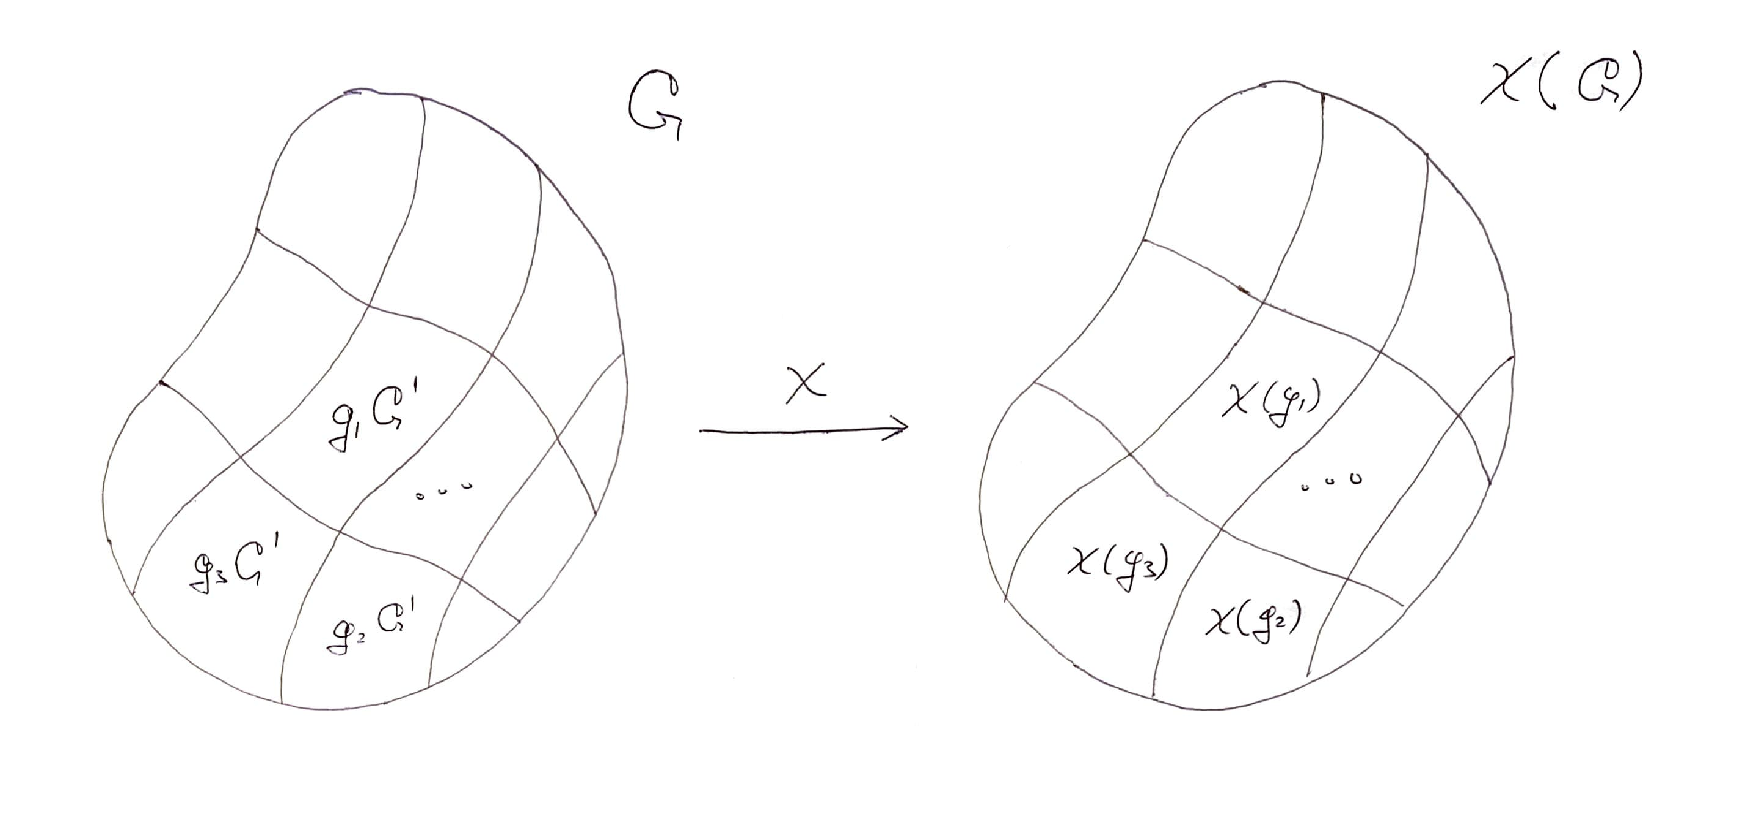
\includegraphics[width=\textwidth]{pictures/chips}
        \caption{}
        \label{img_chi_factor}
    \end{figure}

    \newpage
    Обратно,
    \begin{statement} характер $\chi_{ab}$ однозначно задает $\chi$, как 
        \[\chi = \chi_{ab}\circ \tau\]
    \end{statement}
    Утверждение представляется очевидным.

    Так, построено взаимооднозначное отображение $t: \chi_{ab} \mapsto 
    \chi_{ab} \circ \tau = \chi$ между характерами группы и ее абелизации 
    (т.е. фактор группы по коммутанту). Покажем, что отображение $t$ является 
    гомоморфизмом (а следовательно и изоморфизмом) линейных пространств.

    Действительно, для любого $g \in G$
        \begin{multline*}
        t(c_1\chi_{ab}^1 + c_2\chi_{ab}^2)(g) 
        = (c_1\chi_{ab}^1 + c_2\chi_{ab}^2) \circ \tau (g) = \\
        = (c_1\chi_{ab}^1 + c_2\chi_{ab}^2) (gG')
        = c_1\chi_{ab}^1 (gG') + c_2\chi_{ab}^2 (gG') = \\
        = c_1\chi_{ab}^1 \circ \tau (g) + c_2\chi_{ab}^2 \circ \tau (g)
        = c_1 t(\chi_{ab}^1)(g) + c_2 t(\chi_{ab}^2)(g).
        \end{multline*}
    Тем самым доказано следующее
    \begin{statement}
        Пространства характеров группы $G$ и ее абелизации $G/G'$ изоморфны. 
        Конкретно, изоморфизм имеет вид:
        \begin{equation}\label{iso_GG'}
            t: G/G' \to G.\quad t: \chi_{ab} \mapsto \chi_{ab} \circ \tau,
        \end{equation}
        где $\tau$ --- канонический гомоморфизм $G \to G/G'$.
    \end{statement}
    
    Последнее утверждение позволяет нам свести задачу изучения характеров
    группы $G$ к рассмотрению характеров на $G/G'$ --- группе, абелевой по 
    определению.

\subsubsection{Абелева группа}
    Итак, пусть некоторая группа $A$ --- абелева. Как задать на ней характер? 
    Нетрудно получить ответ в случае \emph{конечно-порожденных} групп.

    Известно, что для таких групп справедливо разложение
    \footnote{см.\cite{Vinberg} гл.9 \S 1}
    \begin{equation*}\label{A_decomp}
        A \simeq \underbrace{\mathbb{Z} \oplus \ldots \oplus \mathbb{Z}}_{n} 
    \oplus \Tor A = \mathbb{Z}^{n} \oplus \Tor A,
    \end{equation*}
    где $\mathbb{Z}^{n}$ --- \emph{свободная подгруппа},\\
    $\Tor A \doteqdot \{a \in A: ma = 0\text{ для некоторого }m \in 
    \mathbb{Z}, m \ne 0\}$ --- \emph{подгруппа кручения}, причем
    \begin{equation*}\label{TorA_decomp}
        \Tor A \simeq \mathbb{Z}_{p_1} \oplus \ldots \oplus \mathbb{Z}_{p_s},
    \end{equation*}
    где $\mathbb{Z}_{p_i}$ --- циклическая группа порядка $p_i$.
    
    Отсюда
    \begin{equation}\label{G_basis}
        A = 
        \{x_1 e_1 + \ldots + x_n e_n + x_{n+1} f_1 + \ldots + x_{n+s} f_s 
        \:|\: x_i \in \mathbb{Z}\},
    \end{equation}
    где $\{e_i\}_{i=1}^n$ -- базис свободной подгруппы, $\{f_i\}_{i=1}^s$ -- 
    порождающие соответствующих циклических групп. Попутно введем обозначение 
    $\subdim A = n$.

    Пусть теперь задан характер $\chi: A \to \mathbb{C}$, тогда для любого 
    $a \in A$, с учетом \eqref{G_basis} верно
    \begin{multline*}
        \chi(a) = \chi(\alpha_1 e_1 + \ldots + \alpha_n e_n 
        + \alpha_{n+1} f_1 + \ldots + \alpha_{n+s} f_s ) = \\
        = \alpha_1 \chi(e_1) + \ldots + \alpha_n \chi(e_n) 
        + \alpha_{n+1} \chi(f_1) + \ldots + \alpha_{n+s} \chi(f_s),
    \end{multline*}
    но, так как порядок каждого элемента $f_i$ конечен, то $\chi(f_i) = 0$ для 
    всех $i=1 \comdots, s$, и
    \begin{equation}\label{chi_decomp}
        \chi(a) = \alpha_1 \chi(e_1) + \ldots + \alpha_n \chi(e_n).
    \end{equation}
    
    Тем самым доказано
    \begin{statement}
        Для конечно-порожденной группы $A$ пространство характеров 
        $X(A) = \{\chi: A \to \mathbb{C}: 
        \chi(a + b) = \chi(a) + \chi(b)\}$ имеет размерность
        \begin{equation}
            \dim X(A) = \subdim A.
        \end{equation}
    \end{statement}

\qed
\begin{thebibliography}{0}
    \bibitem{MacLane} Маклейн~С.
        \emph{"<Категории для работающего математика">}. Изд-во ФизМатЛит, Москва, 2004.
    \bibitem{Vinberg} Винберг~Э.~Б.
        \emph{"<Курс алгебры">}. Изд-во МЦНМО, Москва, 2014.
\end{thebibliography}

\end{document}